\chapter{METODOLOGIAS DE DESENVOLVIMENTO}
\label{cap:02}

A medida que o \textit{software} começou a ganhar mais importância na vida das pessoas, as empresas tiveram que investir em modelos que melhoram sua capacidade de produção em um mercado que se torna cada vez mais competitivo, como relata \citeonline{4222727}. Não é incomum projetos complexos de \textit{software} precisarem ser executados durante um período de tempo para terem sucesso e até fazerem sentido. Um sistema de análise de candidatos a uma eleição, por exemplo, não teria sentido se ficasse pronto depois que a eleição tivesse acabada. Os modelos de desenvolvimento auxiliaram essas empresas a entenderem melhor a dinâmica de desenvolvimento e ajudaram a desenvolver projetos no melhor custo, prazo e qualidade possível. Nesse capítulo são vistos alguns modelos de desenvolvimento, alguns ainda utilizados, e outros que estão em desuso, mas que representaram grande importância histórica para evolução do que há disponível hoje. Esse capítulo tem como objetivo abordar alguns modelos de processo tradicionais: como o cascata, incremental e RUP. Logo depois, são vistos algumas metodologias ágeis que são utilizadas no mercado como SCRUM, XP, LSD etc. 
%A medida que o \textit{software} foi ganhando maior impotância na vida das pessoas e das empresas, tornou-se necessária a criação de \textit{softwares} de maneira repetida, mais rápida e com qualidade. Pode-se dizer que esses modelos {, tanto no mercado como no meio acadêmico, surgiram modelos que foram criados para organizar e melhorar o fluxo de desenvolvimento de \textit{software}.

\section{PROCESSO DE SOFTWARE}

Quando um projeto de \textit{software} precisa ser executado, os engenheiros e seus gerentes utilizam um processo de \textit{software}. Um processo de \textit{sofware}, como define \citeonline{pressman:11}, é um conjunto de atividades de trabalho, ações e tarefas realizadas a fim de produzir algum artefato de \textit{software}. Cabe ressaltatar que a palavra artefato foi empregada de forma a dar enfase de que não apenas o \textit{software} em si é produzido, mas a documentação etc. Um processo, que muitas vezes é adaptado a algum tipo de projeto, possui uma metodologia de apoio, a qual possui atividades, as quais por sua vez possuem ações e tarefas atreladas.

% \begin{figure}[hb]
% \begin{center}
% \caption{Visão de alto nível de um processo de software}
% \label{fig:02}
% 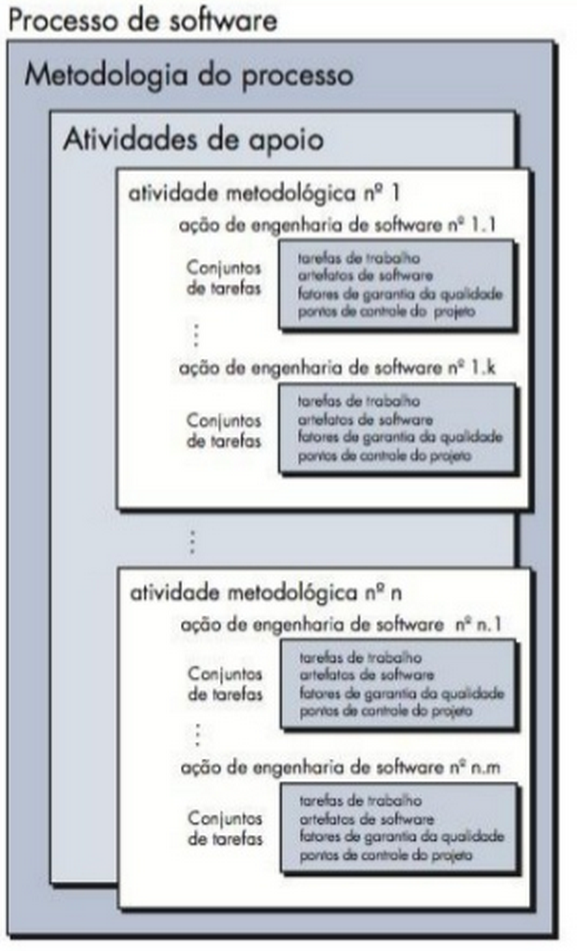
\includegraphics[height=9cm]{assets/processo} \\
% \fonte{\citeauthoronline{pressman:11}, \citeyear{pressman:11}.}
% \end{center}
% \end{figure}

Geralmente no que tange as atividades do projeto, o engenheiro e os gerentes possuem uma flexibilidade para utilizar as atividades que acharem mais coerente, sendo as principais comunicação, planejamento, modelagem, construção e entrega. Atividades de apoio, e.g. acompanhamento e controle do projeto, administração de risco e garantia de qualidade, gerenciamento de configuração, revisões técnicas etc., são também empregadas durante o processo \cite{pressman:11}. 

As atividades de uma metodologia necessitam de um fluxo de processo. O fluxo de processo descreve a sequência das atividades e seus relacionamentos entre si. A Figura \ref{fig:02} mostra um exemplo de um fluxo de processo linear, ou seja, cada atividade é executada em sequência, uma após a outra. Assim, o software só ficaria pronto depois de passar pelas 4 etapas iniciais. Esse é o fluxo de processo utilizado pelo modelo em cascata por exemplo, o qual será visto mais adiante. 

\begin{figure}[htb!]
\begin{center}
\caption{Fluxo de processo linear}
\label{fig:02}
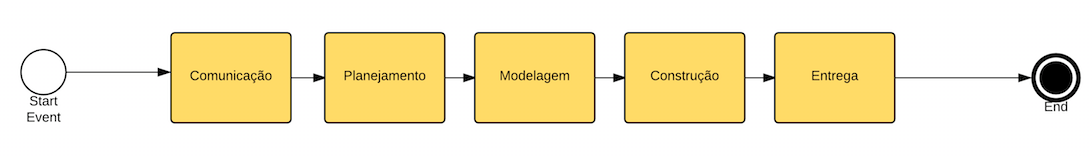
\includegraphics[height=2cm]{assets/linear} \\
\fonte{Adaptado de \citeauthoronline{pressman:11}, \citeyear{pressman:11}.}
\end{center}
\end{figure}


Outro fluxo de processo existente é o evolucionário, utilizado bastante em metodologias ágeis. Nele, um \textit{software} é feito através de várias entregas pontuais. Cada volta no ciclo produz uma versão do \textit{software} mais completa. É ideal para projetos com requisitos não muito bem definidos e complexos. Sua vantagem é que o cliente pode participar e dar \textit{feedback} constantemente e ver como o produto está ficando. A Figura \ref{fig:03} ilustra esse processo.

\begin{figure}[htb!]
\begin{center}
\caption{Fluxo de processo evolucionário}
\label{fig:03}
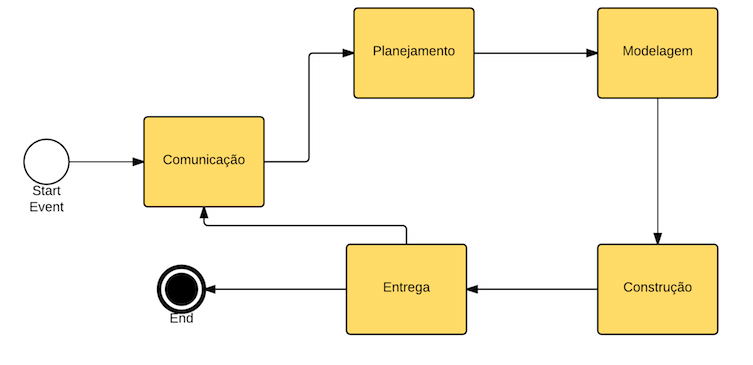
\includegraphics[width=10cm]{assets/evolucionario} \\
\fonte{Adaptado de \citeauthoronline{pressman:11}, \citeyear{pressman:11}.}
\end{center}
\end{figure}

Finalmente há o fluxo de processo paralelo, o qual se diferencia dos outros por possibilitar que uma ou mais tarefas possam ser executadas em paralelo. Na Figura \ref{fig:04} é mostrado um exemplo de fluxo paralelo. Neste ciclo, poderia-se estar na modelagem e na construção ao mesmo tempo, por exemplo.

\begin{figure}[htb!]
\begin{center}
\caption{Fluxo de processo paralelo}
\label{fig:04}
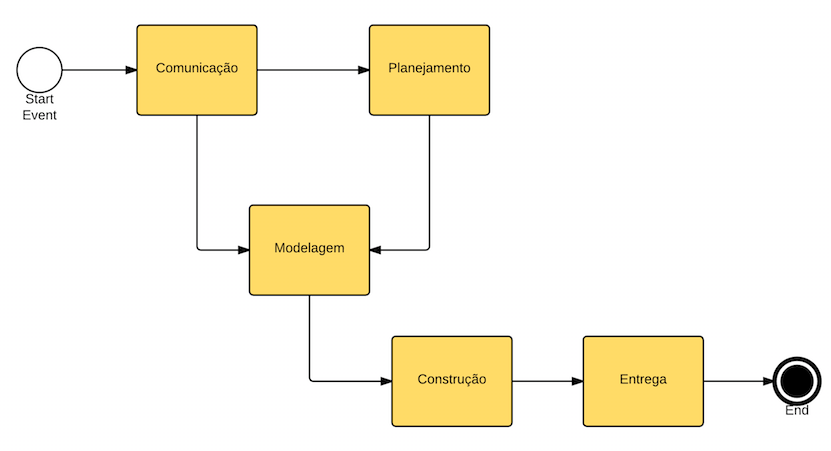
\includegraphics[width=10cm]{assets/paralelo} \\
\fonte{Adaptado de \citeauthoronline{pressman:11}, \citeyear{pressman:11}.}
\end{center}
\end{figure}

Na próxima seção são vistos alguns modelos de desenvolvimento, que como visto, empregam algum fluxo de processo.

\section{MODELOS DE DESENVOLVIMENTOS TRADICIONAIS}

Como visto na seção anterior, os modelos de desenvolvimento estão atralado a um ou mais fluxos de processo. Nesta seção são vistos alguns modelos de desenvolvimento que foram utilizados pela indústria de software e outros que ainda são amplamente utilizados. Como há muitos modelos, são descritos os principais segundo \citeonline {pressman:11}.

\subsection{Cascata}
\label{sec:cascata}

O modelo de desenvolvimento cascata é o ciclo de desenvolvimento mais simples possível. Ele começa basicamente com o levantamento de requisitos por parte do cliente e depois com as etapas de planejamento, modelagem e construção de forma sequencial. Não é possível ir de uma etapa para outra ou pular alguma etapa no processo. Seu fluxo de processo segue o mesmo princípio da Figura \ref{fig:02} e por isso não é mostrado. Dentro da etapa de comunicação há atividades como início do projeto e levantamento de requisitos. Na etapa de planejamento, há atividades como estimativas de cronograma e acompanhamento. Na modelagem há a análise do projeto. A construção possui as atividades de codificação e testes e finalmente no emprego atividades como entrega, suporte e \textit{feedback}.

\citeonline{pressman:11} descreve alguns pontos negativos da utilização desse processo como a natureza incerta de projetos de \textit{software} que fazem com que as necessidades sejam difíceis de serem traduzidas de uma vez. Além disso, como mencionado anteriormente o cliente precisa esperar pacientemente até possuir uma versão funcional: que as vezes pode estar bem longe do que ele pediu. Se os requisitos são muito bem definidos e o trabalho deve ser realizado até o final de forma linear, talvez esse seja um processo ideal. 

\subsection{Modelo de Processo Incremental}

Ao contrário do modelo em cascata, que geralmente é utilizado em projetos cujos requisitos estão bem definidos, o modelo incremental fica no meio termo. Ele é geralmente empregado em projetos cujos requisitos estão razoavelmente definidos. O modelo combina elementos do fluxo de processo linear e paralelo. Em cada incremento é disponibilizada uma versão aprovada e utilizável do \textit{software} para o usuário, de forma que os futuros incremento serão responsáveis por implementar novas funcionalidades ou expanções das fucionalidades existentes. Como explana \citeonline{pressman:11}, os primeiros incrementos são versões funcionais, mas não completas do \textit{software}, assim esse modelo é muito útil quando não há diposponível mão de obra suficiente para entrega de um produto no prazo ou para projetos com baixo orçamento, pois se o sistema for bem aceito, novos incrementos podem ser feitos e mais pessoas podem ser adicionadas ao projeto.


A Figura \ref{fig:05} ilustra o modelo do processo incremental. Pode-se observar que conforme o tempo passa, linha horizontal, novos incrementos são feitos e consequentemente novas funcionalidades e recursos são liberados.

\begin{figure}[htb!]
\begin{center}
\caption{Fluxo de processo incremental}
\label{fig:05}
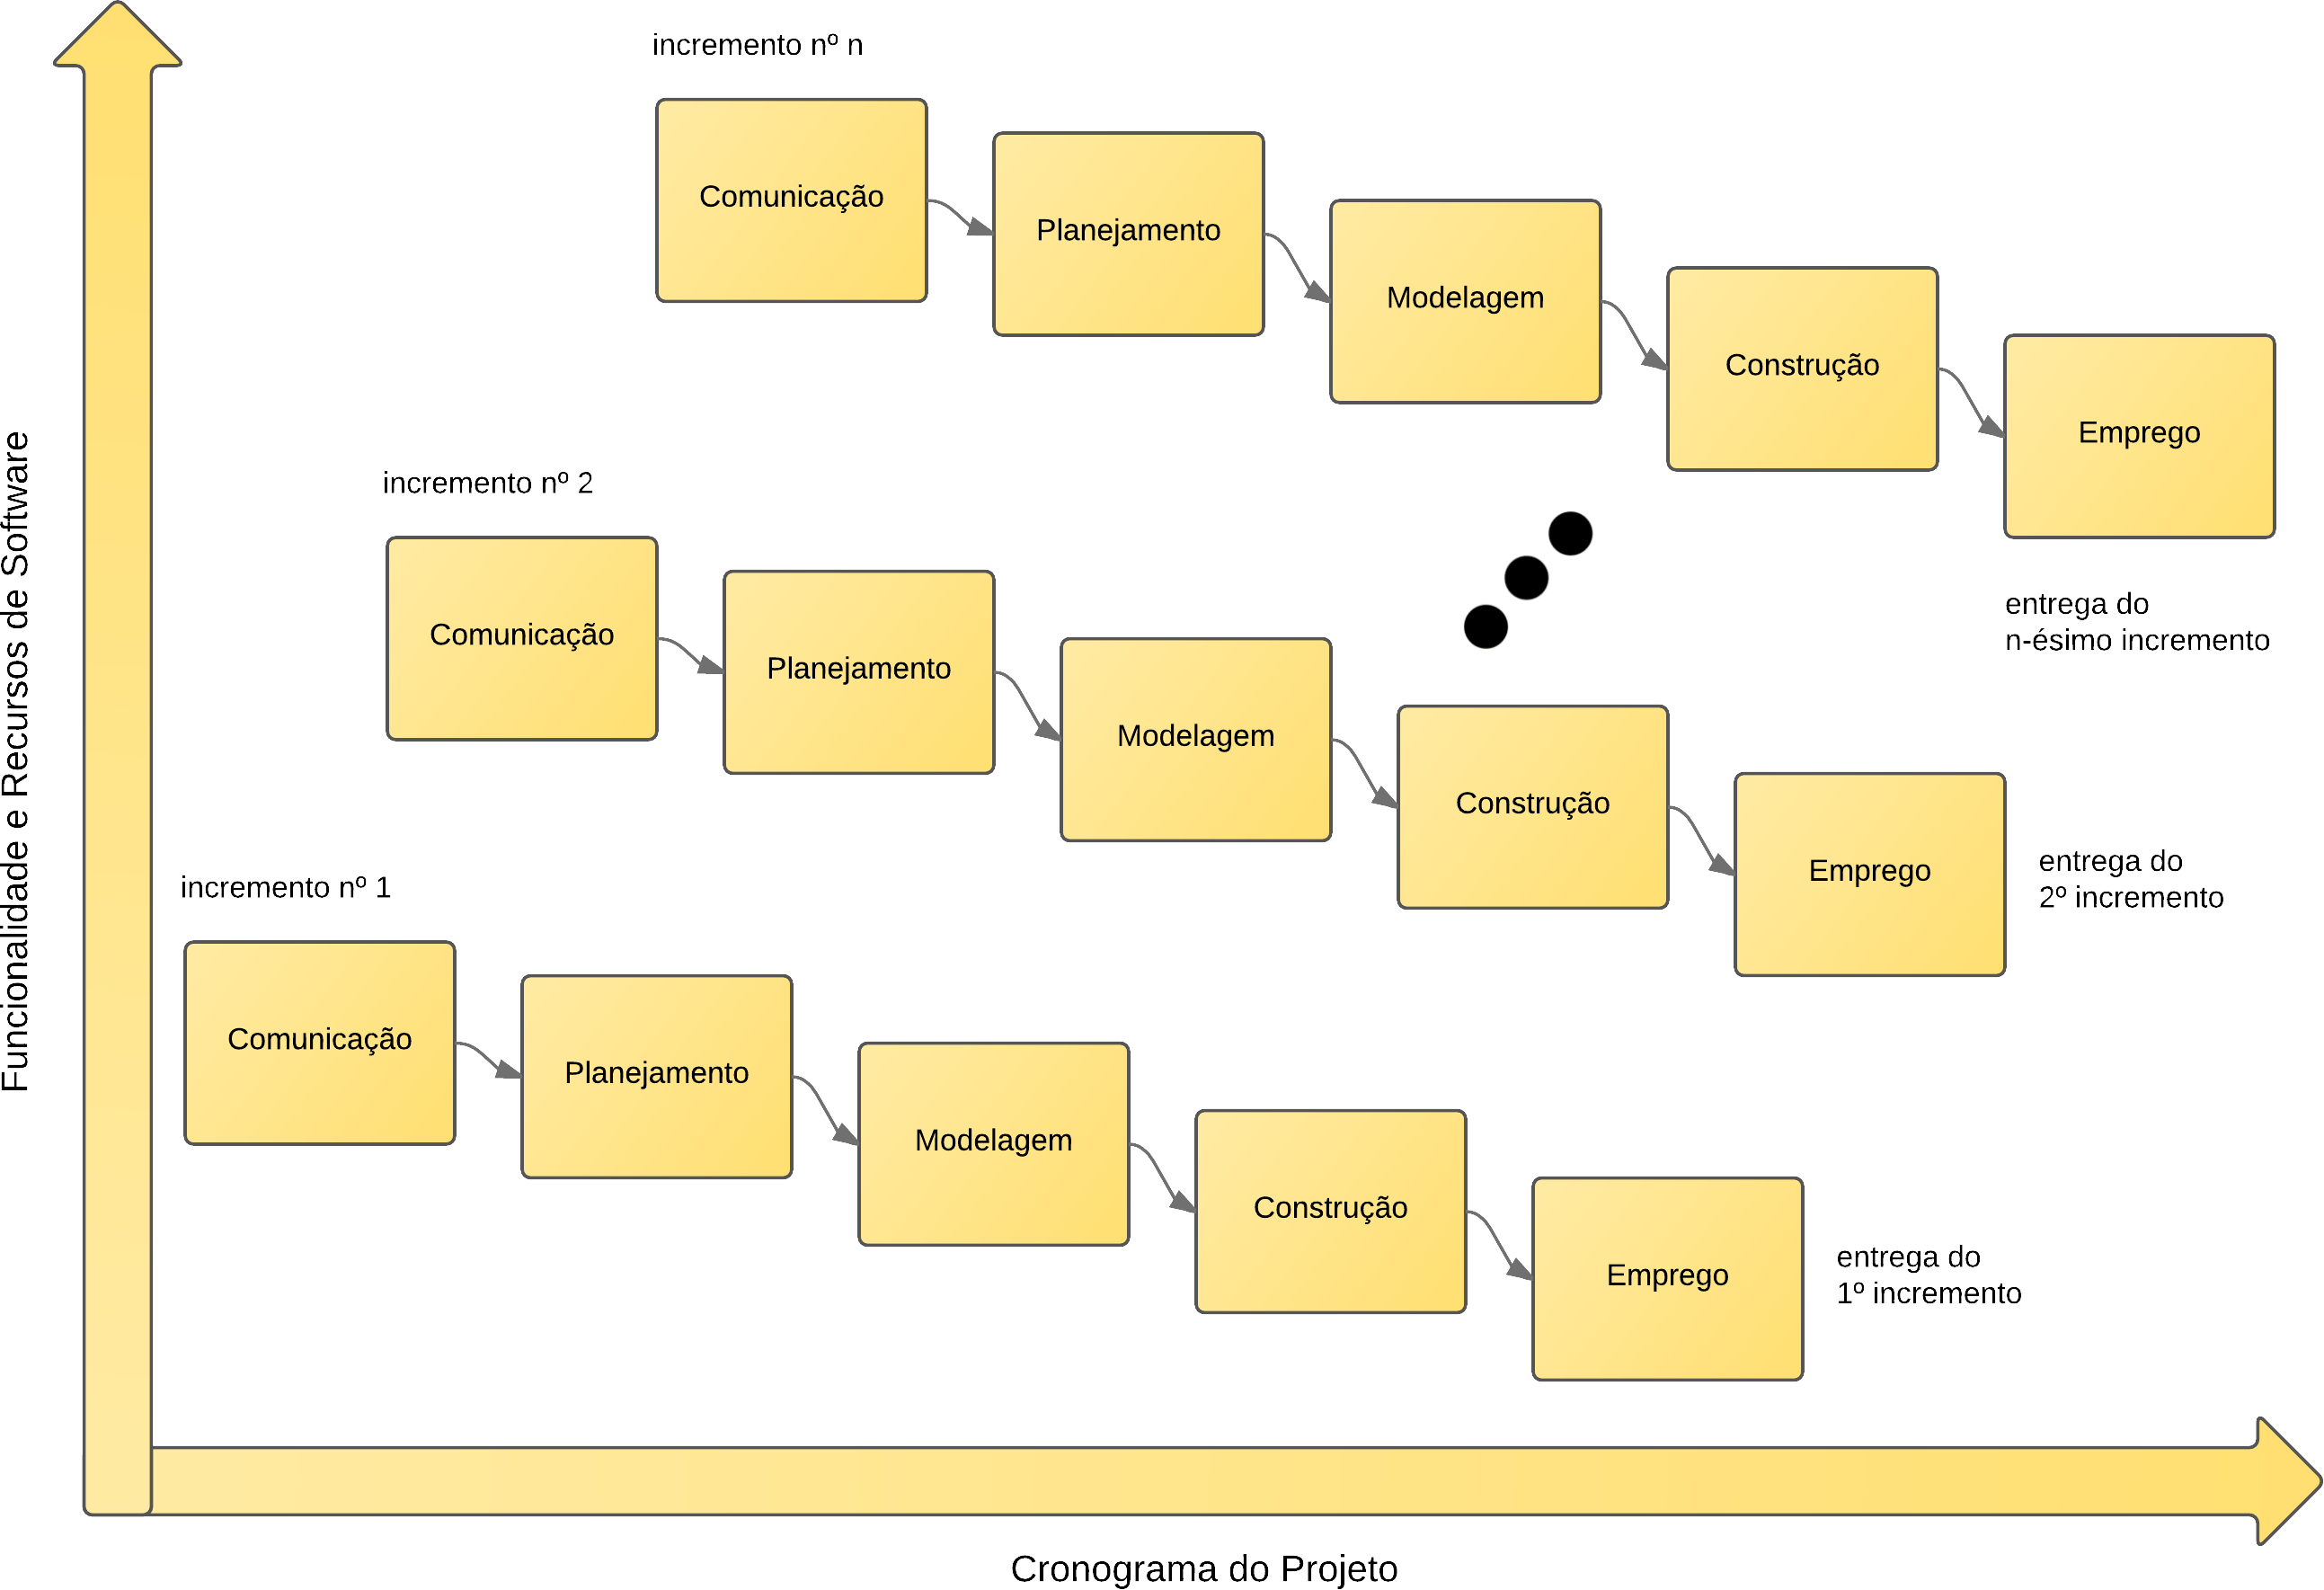
\includegraphics[width=10cm]{assets/incremental} \\
\fonte{Adaptado de \citeauthoronline{pressman:11}, \citeyear{pressman:11}.}
\end{center}
\end{figure}

\subsection{Modelo de Processo Evolucionário}
\label{sec:espiral}
A medida que o mercado demanda que produtos complexos tenham que ser desenvolvidos em um curto prazo, uma versão limitada pode ser desenvolvida para atender as necessidades de negócio. Há projetos cujos detalhes do sistema não estão muito definidos a longo prazo, devido a complexidade, e assim faz-se necessário o uso de um modelo evolucionário. Os modelos evolucionários são iterativos, ou seja, permitem que versões cada vez mais completas do sistema sejam entregues. Dois modelos de processos comuns são o modelo de prototipação e evolucionário. 

O modelo de prototipação pode ser usado como um processo dentro de qualquer outros dos modelos citados anteriormente (cascata, incremental etc.) ou sozinho. Sua vantagem é que devido a incerteza de um projeto complexo, um protótipo pode ser construído a fim de validar a aplicação que será construida e até mesmo levantar requisitos através do \textit{feedback} dos \textit{stakeholders}\footnote{O palavra inglesa \textit{stakeholders} denota qualquer pessoa interessada no projeto.}. Um dos problemas com essa abordagem, segundo \citeonline{pressman:11}, é que os \textit{stakeholders} podem enxergar o sistema como algo operacional, e assim, algo que foi feito rapidamente apenas como protótipo (sem foco em qualidade) pode ser utilizado, tornando o código sem qualidade e não performático. A Figura \ref{fig:06} mostra o paradigma da prototipação.


\begin{figure}[htb!]
\begin{center}
\caption{Paradigma da prototipação}
\label{fig:06}
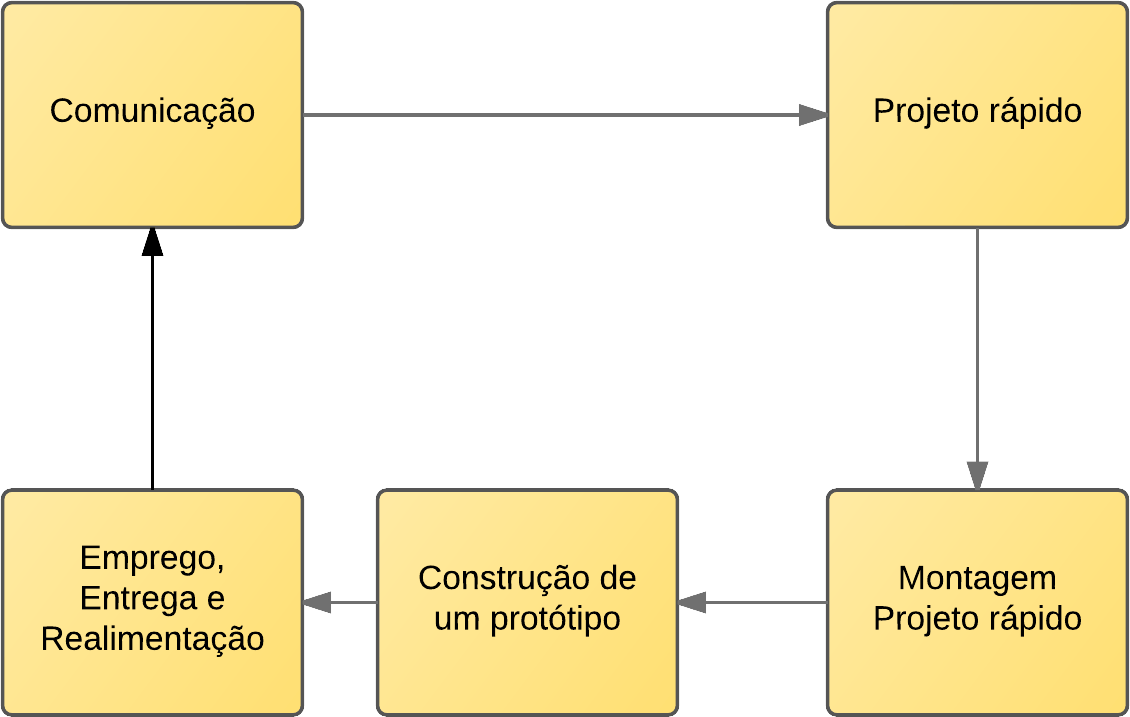
\includegraphics[width=10cm]{assets/prototipacao} \\
\fonte{Adaptado de \citeauthoronline{pressman:11}, \citeyear{pressman:11}.}
\end{center}
\end{figure}

Outro modelo de processo evolucionário é o espiral. Proposto por Barry Boehm, ele agrega a natureza iterativa da prototipação com o modelo em cascata. Esse modelo fornece uma maneira para construção rápida de várias versões do sistema. Nas primeiras versões, um modelo ou um protótipo é contruido. A partir das futuras iterações, esse protótipo torna-se um sistema cada vez mais completo. A Figura \ref{fig:07} mostra um espiral com 4 atividades, as quais podem ser modificadas pela equipe. O ciclo de desenvolvimento começa no centro e a equipe de desenvolvimento define as etapas (eg. comunicação, planejamento, modelagem, construção etc.). Como dito anteriormente, cada volta no ciclo define uma iteração.

\begin{figure}[htb!]
\begin{center}
\caption{Modelo espiral}
\label{fig:07}
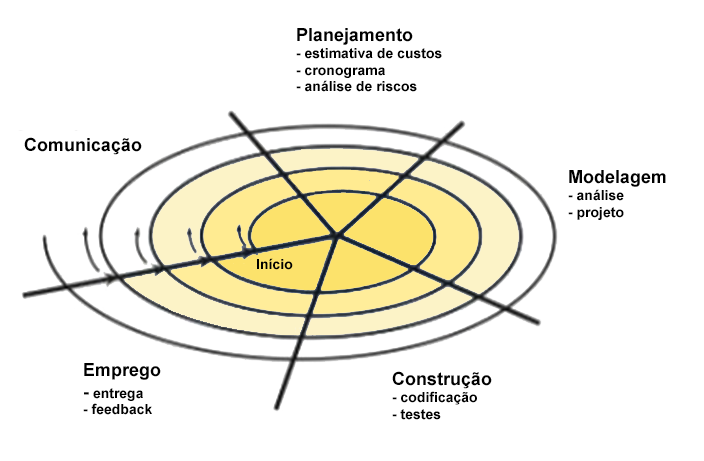
\includegraphics[width=10cm]{assets/espiral} \\
\fonte{Adaptado de  \citeauthoronline{pressman:11}, \citeyear{pressman:11}.}
\end{center}
\end{figure}

\subsection{PSP e TSP}

O processo de \textit{software} pessoal, ou \textit{personal software project}, é uma metodologia de desenvolvimento que encoraja o desenvolvedor a conhecer melhor sobre si mesmo para poder estimar e desenvolver \textit{softwares} com mais qualidade e acertividade no que tange as estimativas. A Figura \ref{fig:08} ilustra a dinâmica do modelo. Nela observa-se que o PSP é composto de \textit{scripts}, ou guias, que dizem as ações que o desenvolvedor deve executar para cada etapa. A medida que o desenvolvedor evolui nas etapas, esses guias podem solicitar que informações sejam adicionadas nos logs. Na fase de codificação, por exemplo, cada erro que você encontra no código e seu tempo de correção é anotado. Ao final do projeto, além de ter o sistema, o desenvolvedor tem um relatório que irá ajudá-lo nas estimativas para futuras funcionalidades desse e de outros projetos \cite{humphrey:00}.

\begin{figure}[htb!]
\begin{center}
\caption{Modelo do PSP}
\label{fig:08}
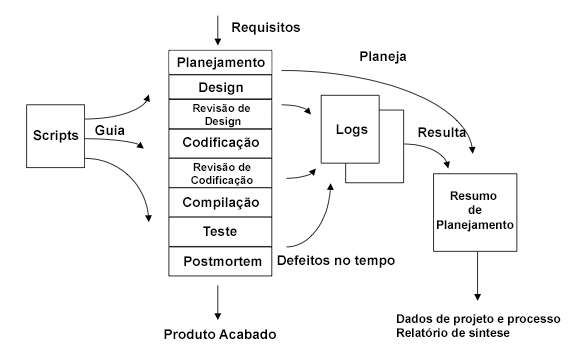
\includegraphics[width=13cm]{assets/psp} \\
\fonte{Adaptado de \citeauthoronline{humphrey:00}, \citeyear{humphrey:00}.}
\end{center}
\end{figure}

\citeonline{humphrey:00} mostra em seu trabalho que a introdução ao PSP/TSP em universidades segue o roteiro da Figura \ref{fig:09}. O curso geralmente possui duração de um semestre e foca na construção de aproximadamente 10 programas. Inicialmente o aluno inicia no que é chamado de PSP 0 (PSP nível 0), o qual ele se utiliza de suas práticas atuais de desenvolvimento e apenas registra o tempo que gastar em cada fase do ciclo de desenvolvimento. Esse processo é melhorado através dos outros níveis até que ele atinja um nível superior e consequentemente aprenda a maioria dos métodos do PSP. No caso de sua aplicação para indústria, há um curso com cerca de 10 programas que levam em torno de 120 a 150 horas divididos em 14 dias.

\begin{figure}[htb!]
\begin{center}
\caption{Níveis do PSP}
\label{fig:09}
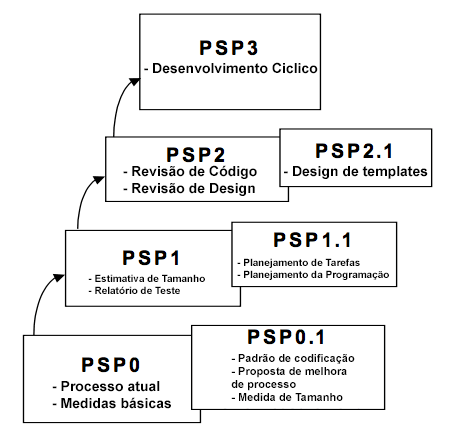
\includegraphics[width=7cm]{assets/psp-nivel} \\
\fonte{Adaptado de \citeauthoronline{humphrey:00}, \citeyear{humphrey:00}.}
\end{center}
\end{figure}

Além do PSP existe o TSP (\textit{team software process}) que é a aplicação do PSP para criar uma equipe de projetos autodirigida. \citeonline{pressman:11} explica que os membros de uma equipe TSP estabelecem objetivos para o projeto, adaptam o processo para atender as expectativas do projeto e trabalham continuamente para aperfeiçoar o precesso de engenharia.

\subsection{Processo Unificado da Rational (RUP)}
\label{sec:rup}

O processo unificado é oriundo da discussão de Ivar Jacobson, Grady Booch e James Rumbaugh sobre a necessidade de um processo de software digirido a casos de uso, centrado na arquitetua, iterativo e iterativo incremental. Assim, o processo unificado utiliza-se de recursos e características de modelos tradicionais de processo de software e alguns dos princípios de metodologias ágeis como comunicação com o cliente. Esse processo é proprietário e foi criado inicialmente pela empresa \textit{Rational Software Development}, qual foi adquirida pela IBM \cite{pressman:11} \cite{machado:13}. 

O processo unificado é composto segundo \citeonline{machado:13} por:

\begin{itemize}
	\item \textbf{Papéis}: define quem é responsável por uma tarefa;
	\item \textbf{Artefatos}: o que será gerado durante cada tarefa. Pode ser um documento, um modelo do sistema etc;
	\item \textbf{Atividades}: o que cada responsável executa para atingir os objetivos do projeto e
	\item \textbf{Fluxo de atividades}: orienta a execução das atividades.
\end{itemize}

Além dos papéis, o RUP possui práticas que visam resolver problemas que ameaçam projetos como: alta complexidade, falta de definição formal de um processo de gerenciamento de mudanças, inconsistências não detectadas em requisitos (design e implementação), testes insuficientes, controle subjetivo, falha ao atacar riscos do projeto, comunicação ambigua e imprecisa e automação insuficiente. A seguir são vistas as práticas de acordo com \citeonline{machado:13}.

\begin{enumerate}
\item \textbf{Desenvolvimento iterativo}: Utilização do modelo em espiral e a construção do \textit{software} se em iterações. Para mais informações sobre o modelo, consulte a seção \ref{sec:espiral}.
\item \textbf{Gerenciar os requisitos}: Consiste em elicitar, organizar e documentar a funcionalidade e restrições do \textit{software}.
\item \textbf{Usar arquitetuas baseadas em componentes}: Sistema é organizado em módulos coesos e fracamente acoplados. Um modelo pode ser desenvolvido por um terceiro, aproveitado de outro projeto e desenvolvido desde o início.
\item \textbf{Modelar software visualmente}: Utilização da modelos (e.g UML) para descrever o sistema de forma não ambigua.
\item \textbf{Verificar qualidade do software continuamente}: Testes em cenários de utilização a cada incremento.
\item \textbf{Controlar mudanças}: Cada mudança do \textit{software} necessita de um requisito de mudança que descreve criteriosamente as mesmas. 
\end{enumerate}
  
Além disso, o RUP é um processo orientado a casos de uso e pode ser adaptado (com restrições) pela organização. A Figura \ref{fig:rup} ilustra a estrutura do RUP. O projeto é dividido nas fases de iniciação, elaboração, construção e transição. Cada é composta por disciplinas que dão diretrizes de como proceder. Cada fase pode ter uma ou mais iterações. Observa-se na Figura \ref{fig:rup} que inicialmente os maiores esforços estão na modelagem, requisitos e análise. A fase de iniciação é fundamental para mitigar os riscos. A elaboração é responsável pelo planejamento das atividades e recursos necessários para o projeto, especificação detalhada dos requisitos e projeto de arquitetura. A fase de construção em como objetivo evoluir o sistema que está sendo proposto. A transição marca a entrega para os usuários de um produto quase pronto com apenas questões de empacotamento, entrega, treinamento, suporte e manutenção.


\begin{figure}[htb!]
\begin{center}
\caption{Estrutua do RIP}
\label{fig:rup}
\includegraphics[width=10cm]{assets/rup} \\
\fonte{Adaptado de \citeauthoronline{machado:13}, \citeyear{machado:13}.}
\end{center}
\end{figure}

\section{DESENVOLVIMENTO ÁGIL}
\label{sec:agile}
O desenvolvimento ágil surgiu através da assinatura do ``Manifesto para o Desenvolvimento Ágil de Software'' por dezesseis desenvolvedores, autores e consultores da área de \textit{software} e Kent Beck. Esse manifesto tinha como objetivo quebrar o velho conceito que havia em relação ao desenvolvimento dos projetos de \textit{software}, os quais possuiam muitos formalismos, documentação excessiva etc. Pode-se dizer que o movimento ágil é uma resposta ao mercado que se tornou, com o passar do tempo, mais competitivo e exigiu que projetos fossem executados rapidamente e ao mesmo tempo com capacidade de se adaptar as mudanças de forma rápida e menos custosa \cite{pressman:11}.  

O manifesto ágil possui os seguintes valores segundo \citeonline{agilemanifesto:15}:

\begin{citacao}
\begin{itemize}
	\item Indivíduos e iterações sobre processos e ferramentas;
	\item Software operacional acima de documentação completa;
	\item Colaboração dos clientes acima de negociação contratual e
	\item Respostas a mudanças acima de seguir um plano.
\end{itemize}
\end{citacao}

Além dos valores pregados pelo manifesta, ele possui os seguintes princípios segundo \citeonline{agilemanifesto:15}:

\begin{citacao}
\begin{itemize}
	\item Nossa maior prioridade é satisfazer o cliente através da entrega contínua e adiantada de software com valor agregado;
	\item Mudanças nos requisitos são bem-vindas, mesmo tardiamente no desenvolvimento. Processos ágeis tiram vantagem das mudanças visando vantagem competitiva para o cliente;
	\item Entregar frequentemente software funcionando, de poucas semanas a poucos meses, com preferência à menor escala de tempo;
	\item Pessoas de negócio e desenvolvedores devem trabalhar diariamente em conjunto por todo o projeto;
	\item Construa projetos em torno de indivíduos motivados. Dê a eles o ambiente e o suporte necessário e confie neles para fazer o trabalho;
	\item O método mais eficiente e eficaz de transmitir informações para e entre uma equipe de desenvolvimento é através de conversa face a face;
	\item Software funcionando é a medida primária de progresso;
	\item Os processos ágeis promovem desenvolvimento sustentável. Os patrocinadores, desenvolvedores e usuários devem ser capazes de manter um ritmo constante indefinidamente;
	\item Contínua atenção à excelência técnica e bom design aumenta a agilidade;
	\item Simplicidade -- a arte de maximizar a quantidade de trabalho não realizado -- é essencial;
	\item As melhores arquiteturas, requisitos e designs emergem de equipes auto-organizáveis e
	\item Em intervalos regulares, a equipe reflete sobre como se tornar mais eficaz e então refina e ajusta seu comportamento de acordo.
\end{itemize}
\end{citacao}

Nas próximas seções são vistos alguns processos ágeis utilizados no mercado.

\subsection{Extreme Programming -- XP (Programação Extrema)}

\textit{Extreme Programming} é uma metodologia ágil de desenvolvimento de projetos de \textit{software}, criada por Kent Beck em 1996, ideal para pequenas e médias equipes de desenvolvimento. Como a maioria das metodologias ágeis, é uma metodologia com foco em projetos cujos requisitos não são bem definidos no início do projeto e cujos requisitos tendem a mudar constantemente. As principais características da XP segundo \citeonline{macedo:12} são: 

\begin{itemize}
	\item \textit{Feedback} constante;
	\item Abordagem incremental e
	\item Encojajamento da comunicação entre as pessoas envolvidas.
\end{itemize}

Por abordagem incremental entende-se o modelo discutido anteriormente nesse capítulo, ou seja, a evolução do sistema se dá através de escolhas de funcionalidades principais do sistema, as quais são cada vez melhoradas e extendidas conforme o projeto evolui. Em cada final de incremento, a equipe tem um sistema ``utilizável'', o qual os \textit{stakeholders} podem validar e dar opiniões: o que facilita sua mudança em relação aos requisitos e encora a comunicação como identificado por \citeonline{macedo:12}.

A XP é uma metodologia de projetos de \textit{software} que dá preferência a utilização do paradigma de orientação a objetos e pequenas equipes de até 12 desenvolvedores. Além disso, a XP é uma metodologia flexível que pode ser adaptada a um projeto conforme a necessidade. A metodologia possui divisões, as quais possuem características atreladas. As divisões são: valores, equipe e prática, as quais são detalhadas mais adiante segundo \citeonline{macedo:12}. A estrutura da metodologia é observada na Figura \ref{fig:10}.

\begin{figure}[htb!]
\begin{center}
\caption{Estrutura da XP}
\label{fig:10}
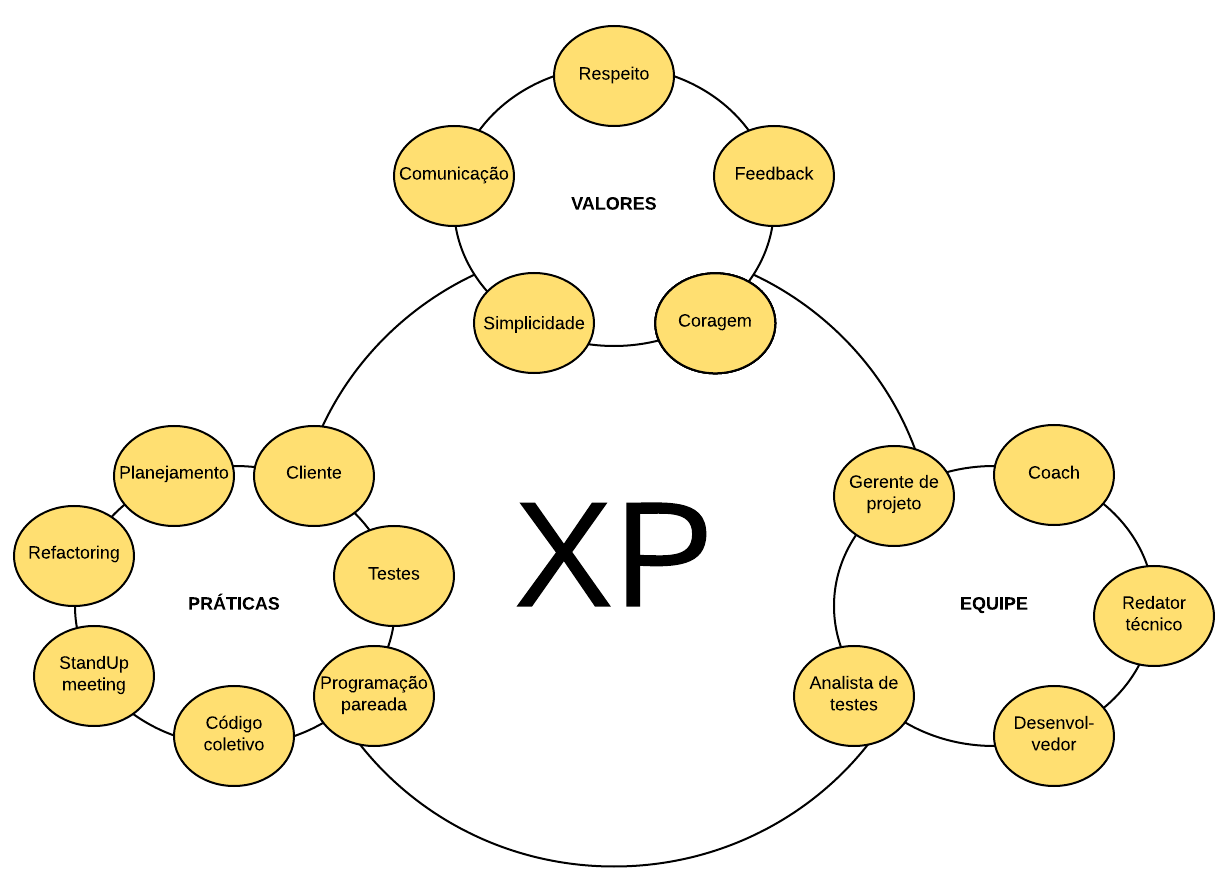
\includegraphics[width=14cm]{assets/xp} \\
\fonte{Adaptado de \citeauthoronline{macedo:12}, \citeyear{macedo:12}.}
\end{center}
\end{figure}

Para que uma equipe de desenvolvimento diga que construiu um \textit{software} utilizando XP, é necessário que a equipe siga os seus valores sob a forma de diretrizes, mesmo que ela adapte a metodologia com sua necessidade. 

Os valores da XP, como dito anteriormente e mostrado na Figura \ref{fig:10}, são comunicação, \textit{feedback}, simplicidade e coragem. Na questão de comunicacão, é importante que haja a comunicação entre os desenvolvedores e o cliente de forma direta (até mesmo face a face). O cliente deve tornar-se e sentir-se peça fundamental no processo de desenvolvimento. 

Outro valor importante da XP é o \textit{feedback}. Por utilizar uma abordagem incremental, é fundamental que a comunicação flua por parte dos desenvolvedores com o cliente, assim como do cliente para os desenvolvedores. A cada liberação do incremento de \textit{software}, o cliente pode testar o que foi produzido para validar e ajudar os desenvolvedores no rumo que o sistema deve tomar. 

A simplicidade é outro valor importante da XP. Deve-se implementar uma funcionalidade da forma mais simples possível para funcionar. O XP, como uma metodologia ágil, parte do princípio de que os requisitos são incertos e estão sempre mudando, assim deve-se sempre pensar no agora e deixar funcionalidades que somente serão utilizadas no futuro para depois. O foco está somente em funcionalidades que agregam valor ao cliente no momento.

Outro valor importante da XP é a coragem. Toda a equipe (desenvolvedores e equipe de projeto) devem tomar atitudes complexas e de alto risco. Alguns problemas que surgem devem ser pensados durante ou antes do desenvolvimento. Todo projeto deve ser discutido e analisado ao receber a proposta do cliente. A coragem é um valor que deve ser tomado em qualquer alteração ou sugestão de alteração no escopo do produto, processo e também nas pessoas. O desenvolvimento deve seguir um ritmo sustentável e todos os artefatos (e.g. documetação, fontes etc.) devem estar disponíveis para os membros da equipe. Outro fator importante é a refatoração, ou seja, os desenvolvedores e projetistas devem tomar um tempo para melhorar o código ou arquitetura do sistema. O contato dos desenvolvedores com o cliente é fundamental nessa metodologia para gerar \textit{feedback}. Testes automatizados e programação em pares (com um codificando e outro revisando) são encorajados também. O respeito é outro valor fundamental que faz com que haja respeito entre o cliente e a equipe de desenvolvimento para estimular a crítica e sua aceitação de ambas as partes.

Além dos valores, há boas práticas que os seguidores da XP devem seguir durante o projeto. O padrão de desenvolvimento, depois que a equipe é formada, é imporante para que os desenvolvedores consigam entender o códigos um dos outros. Além disso, a equipe deve escolher a melhor linguagem de programação e as ferramentas que se adequam melhor ao projeto que vai ser construido. A programação deve seguir um \textit{design} mais simples possível, pois os requisitos sempre mudam em projetos incertos e seu custo é alto. Quanto mais simples um código é, mais fácil sua manutenção. 

O cliente é um participante ativo na construção do projeto. O incremento de \textit{software} começa com a história de usuário (feita juntamente com o cliente), a qual será quebrada em atividades. Todas as histórias são priorizadas pelo cliente, de modo que as funcionalidades mais importantes para o sistema sejam feitas em primeiro lugar. Todos os dias é realizada uma reunião chamada de \textit{stand up meeting}, ou reunião em pé, para discutir o que foi feito ontem, os problemas e as histórias que serão desenvolvidas por cada um. As práticas de \textit{pair-programming} (programação em pares), refatoração de código, testes (unitário ou aceitação), metáfora (palavras que facilitam comunicação com o cliente), ritmo sustentável (carga horária de no máximo 40 horas semanais), integração contínua (toda equipe sabe o que foi desenvolvido e o impacto da funcionalidade com o sistema atual é sempre testado) e \textit{releases} curtos são outras práticas utilizadas pela metodologia.

A equipe de um projeto XP é composta pelo gerente de projeto, o qual é responsável por ser o maior elo entre a equipe de desenvolvimento e o cliente. Prazos, custos, cobranças da equipe e ritmo de trabalho são responsábilidades desse papél. Outro papél importante na XP é o \textit{Coach}, ou técnico, que é um profissional com grande experiência e conhecimento da metodologia. Qualquer dúvida deve ser sanada por esse profissional. O desenvolvedor é o profissional responsável por colocar a ideia em prática. Não há diferença entre um desenvolvedor, analista, projetista. O analista de teste (reponsável por validar o produto) e redator técnico (responsável pela documentacão) completam a equipe.


Além do XP, existe também o IXP(\textit{Industrial Extreme Programming} ou programação extrema industrial. Pode-se dizer que é o XP incorporado ao DNA de uma empresa \cite{ixp:2015}. A IXP difere da XP original por contar com uma maior inclusão de gerenciamento, papel expandido para clientes e técnicas atualizadas. A IXP adiciona as seguintes novas práticas no desenvolvimento conforme \citeonline{pressman:11}:

\begin{itemize}
	\item \textbf{Avaliação imediata}: Feita antes do projeto para verificar se o o ambiente de desenvolvimento é apropriado para IXP, se a equipe é composta por interessados, se existe um programa de qualidade diferenciado que apoia melhora contínua, se existe uma cultura de apoio aos novos valores de uma equipe ágil etc.
	\item \textbf{Comunidade de projeto}: Equivale ao papél de equipe na XP, mas pode ser composta, por exemplo, por um tecnólogo, clientes fundamentais e outros envolvidos que desempenham um papel importante no projeto.
	\item \textbf{Mapeamento de projeto}: Avaliação do projeto pela equipe IXP para verificação da justificativa conforme os objetivos da organização. A verificação da consequência em relação a sistemas ou processos existentes também é feita.
	\item \textbf{Gerenciamento orientado a testes}: Criticos avaliam o estado do projeto frequentemente para obter o progresso. É importante para determinar se os objetivos foram atingidos ou não.
	\item \textbf{Retrospectivas}: Tem como objetivo revisar itens, eventos e lições aprendidas a cada iteração de \textit{software} ou do desenvolvimento da versão completa. Tem como objetivo melhorar o processo de aplicação da IXP.
	\item \textbf{Aprendizagem contínua}: Incentiva as pessoas envolvidas a aprendere novos métodos e técnicas para melhorar qualidade do proceso aplicado.
\end{itemize}

Não obstante a essas características, o IXP modifica a XP no uso da prática de SDD (\textit{story-driven development}). Na SDD, histórias para testes de aceitação são realizadas antes da prática de desenvolvimento. Além disso, é encorajado o uso do DDD (\textit{domain-driven design}), ou seja a construção de um modelo de domínio que representa o pensamento de especialistas sobre um assunto da disciplina. A Figura \ref{fig:ixp} mostra os valores (em vermelho) e práticas da IXP.

\begin{figure}[htb!]
\begin{center}
\caption{Valores e práticas da IXP}
\label{fig:ixp}
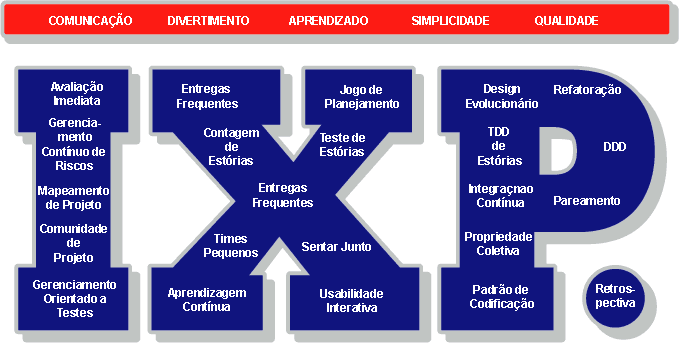
\includegraphics[width=14cm]{assets/ixp} \\
\fonte{Adaptado de \citeauthoronline{ixp:2015}, \citeyear{ixp:2015}.}
\end{center}
\end{figure}

\subsection{Feature Driven Development (FDD)}

A metodologia FDD (\textit{feature driven development})\footnote{O projeto FDD possui um site on o leitor pode obter mais informações \textit{http://bit.ly/1g7hlE1}.} é uma metodologia criada nos anos noventa por Jeff De Luca e Peter Coad para implementação de um sistema bancário internacional que não poderia ser implementado no prazo. Essa metodologia proporciona aos envolvidos no projeto formas de interação e controle fáceis que se traduzem em regras de fácil entendimento e resultados rápidos. Como outras metodologias ágeis, o desenvolvimento é focado em entregas que agregam valor ao cliente através da disponibilização de códigos bem desenvolvidos e testados. Sua utilização se dá tanto em equipes pequenas quanto grandes. Uma característica importante da metodologia é seu foco na qualidade, a qual é enfatizada desde o começo do projeto. Cada nova funcionalidade feita pela equipe deve ser testada e disponibilizada para o usuário. Além disso, a metodologia permite o acompanhamento do progresso do desenvolvimento através de gráficos por parte da equipe e do cliente \cite{macedo:12}. 
Como outras metodologias ágeis, a FDD é centrada em práticas. No FDD são cinco:

\begin{enumerate}
	\item Modelagem de objetos de domínio;
	\item Desenvolvimento por funcionalidade;
	\item Entregas regulares (builds);
	\item Formação da equipe de projeto e
	\item Posse individual do código (classes/\textit{features}).
\end{enumerate}

A modelagem de objetos tem como objetivo estudar, analisar e modelar o sistema que vai ser desenvolvido. Essa atividade convida os responsáveis pelo projeto a realizar tarefas como entrevista, diagramas UML e outros métodos que ajudem os desenvolvedores na implementação \cite{macedo:12}. 

O desenvolvimento por funcionalidade tem como objetivo construir uma lista de funcionalidades a partir dos requisitos. Esses requisitos são classificados de acordo com a área de negócio que pode ser:

\begin{itemize}
	\item Áreas de Negócio (\textit{Business Areas, Major Feature Sets});
	\item Atividades de Negócio (\textit{Business Activities, Features Sets}) e
	\item Passos da Ativididade de Negócio (\textit{Activity Steps, Features}).
\end{itemize}

A entrega regular é caracterizada por manter sempre a entregas para o cliente e trabalhar sempre com o sistema mais recente. Um sistema de versionamento como o GIT ou SVN são extremamente necessários para que isso ocorra.

A metodologia FDD possui cinco papéis: gerente de projeto, arquiteto-chefe/ especialista do negócio, equipe de modelagem/planejamento, programador-chefe e equipe de funcionalidades ``\textit{features}''. O gerente de projetos é o responsável por alocar as pessoas de acordo com suas competências para o projeto e atividades do projeto. Ele é reposponsável por entrar em contato direto com o cliente e extrair os requisitos e acomplanhar o processo de desenvolvimento para que esteja de acordo com o FDD. Um documento contendo as regras de negócio do projeto é feito por ele e os especialistas também para auxiliar os desenvolvedores. O arquiteto-chefe é uma pessoa que deve ser consultada para dúvidas em relação a arquitetura do sistema ou de regra de negócios. Pode não ser necessário, caso o sistema seja muito simples. A equipe de modelagem é responsável por produzir diagramas ou outros artefatos necessários para tornar a implementacão mais fácil. Esse profissional também é responsável por dividiras \textit{features} para a equipe de funcionalide, que são os desenvolvedores propriamente ditos.

A última prática do FDD é a posse individual do código (classe/features). Uma lista de funcinalidades e seus reponsáveis por ela é elaborada. Inspeções regulares através de validação do que foi produzido, gerenciamento de configuração e mudança (através de testes e versionamento) e um relatório/visibilidade de resultados, através de gráficos que indicam o progresso do projeto e suas \textit{features} também são utilizados.   

\subsection{Crystal}

A Crystal, criada por Alistair Cockburn em 1998, é uma família de tecnologias criada com a necessidade de suprimir o mercado de trabalho, o qual tornava-se na época cada vez mais complexo devido a abrangência da utilização de tecnologias e automatização de processos não apenas por grandes empresas, mas por empresas de pequeno e médio porte. A dificuldade de utilização de metodologias tradicionais fez com que uma metodologia que priorizasse a adaptabilidade surgisse. \cite{pressman:11} \cite{macedo:12}

A fim de atingir o objetivo da adaptabilidade, foram criadas várias metodologias com papéis, padrões de processos, produtos de trabalhos e práticas diferentes que pudessem ser escolhidos de acordo com o projeto. \cite{pressman:11}

\citeonline{macedo:12} mostra que a metodologia possui um código genérico com o objetivo de atender vários tipos de projetos, e que a metodologia foi dividida em cores: de acordo com o quão crítico o sistema é.


\begin{table}[htb!]
\centering
\caption{Divisão da família Crystal}
\label{tab:01}
\vspace{0.5cm}
\begin{tabular}{c|c|l}
 
Cores & Nº Desenv. & Em caso de falha \\ 
\hline                               
Clear & 1--6 & Perdem dinheiro, mas recuperam facilmente \\
Yellow & 7--20  & Pedem dinheiro discretamente \\
Orange & 21--40 & Perdem dinheiro substancialmete \\
Red & 41--100 & Perda de dinheiro e até vidas humanas
\end{tabular}
\fonte{\citeauthoronline{macedo:12}, \citeyear{macedo:12}.}
\end{table}

A metodologia Crystal possui, como as outras metodologias, alguns princípios segundo \citeonline{macedo:12}:
\begin{citacao}
\begin{enumerate}
	\item Trabalho face a face com o cliente: considera que envolver o cliente nas iterações e nas decisões é muito mais produtivo;
	\item Peso significa custo: quanto maior a complexidade, maior o custo;
	\item Usar metodologias diferenciadas para equipes maiores;
	\item Mais cerimônias maior criticidade: quanto mais diálogos com os envolvidos melhor;
	\item Comunicação eficiente (\textit{feedback}) é melhor que entregas que não funcionam;
	\item Habitabilidade: tolerância em lidar com seres humanos e
	\item Eficiência no desenvolvimento.
\end{enumerate}
\end{citacao}

A metodologia Crystal possui, segundo \citeonline{macedo:12}, além de seus princípios alguns pensamentos ou filosofias por trás. Num projeto de \textit{software} é importante considerar que cada pessoa trabalha de maneira diferente da outra, assim as limitações de cada um devem ser consideradas em uma empresa com muitos projetos. Outro pensamento é que mesmo que um projeto de \textit{software} seja da mesma área ou tipo, eles podem diferir em necessidades. Além disso, a metodologia, como muitas metodologias ágeis, consideram o desenvolvimento um projeto um processo social que envolve intensa comunicação dos envolvidos, assim é sempre importante também ouvir ideias de usuários (mesmo que inequívoca e inviável no momento). Foco na qualidade que agrega valor ao negócio, consideração de novas técnicas e tecnologias são também importantes em uma área que está em constante evolução e mudança. Por fim, a melhoria do processo vem, em suma, através da experiência da metodologia nos projetos. Na Figura \ref{fig:11} é mostrado o ciclo de vida dessa família de metodologia que é baseado em integrações. Todo o processo deve funcinar de forma cíclica com um time de qualidade que siga as filosofias e princípios.

A equipe da metodologia crystal vai depender complexidade (como visto na Tabela \ref{tab:01}). Caso a equipe seja menor, alguns membros podem assumir mais de uma função. O patrocinador é reponsável pelo investimento financeiro do projeto. O coordenador do projeto possui o papel de definir as entregas e entrar em contato com o patrocinador. Analistas de negócios, usuário \textit{stakeholder} (um usuário do sistema pelo menos), \textit{designer/projetista} (responsável pela arquitetura e elementos de IHC), programadores, testadores (para teste de regressão) e redatores (responsáveis por documentar atas, tabular questinários e entrevistas) são outros participantes desse processo \cite{macedo:12}. 


\begin{figure}[htb!]
\begin{center}
\caption{Ciclo de vida da família de metodologia Crystal}
\label{fig:11}
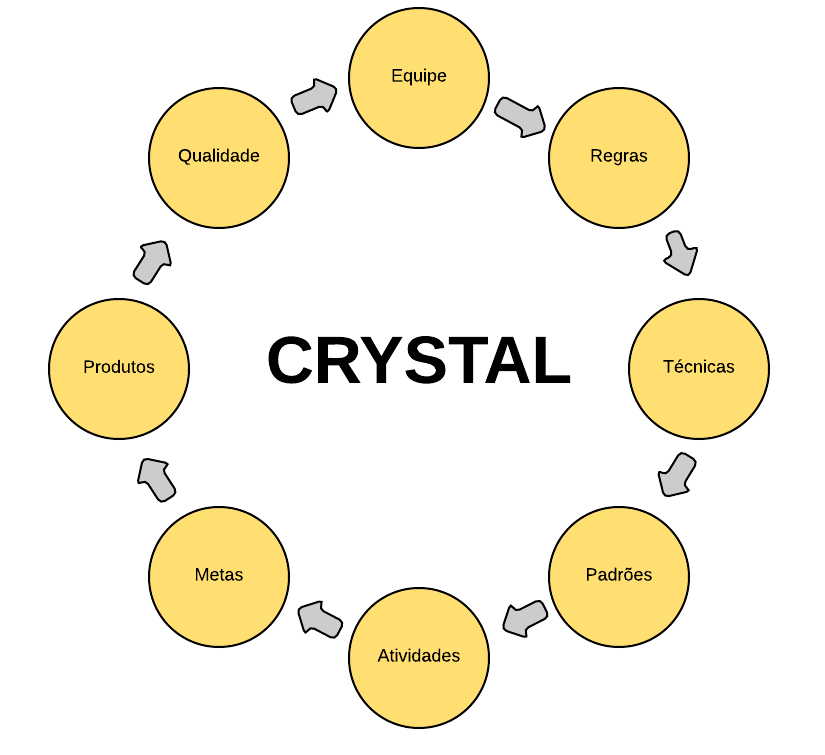
\includegraphics[width=10cm]{assets/crystal} \\
\fonte{Adaptado de \citeauthoronline{macedo:12}, \citeyear{macedo:12}.}
\end{center}
\end{figure}

\subsection{Processo Unificado Ágil (UAP)}

O processo unificado ágil (ou em inglês \textit{Agile Unified Process}) é uma abordagem híbrida criada por Scott Ambler através da combinação do RUP (visto na seção \ref{sec:rup}) com métodos ágeis. Através da combinação de metodologias, criou-se um \textit{framework} capaz de ser aplicado em pequenos e grandes projetos de \textit{software}. Assim, todos os princípios do movimento ágil (visto na seção \ref{sec:agile}) foram agregados ao AUP.
Quando criado por Ambler, o UAP foi centrado nos seguintes princípios segundo \citeonline{edeki:13}:

\begin{itemize}
	\item A maioria das pessoas não lêem documentações detalhadas, no entanto elas precisam de direção e treinamento;
	\item O projeto deve ser descrito de forma simples em algumas páginas;
	\item O AUP deve estar em conforme com o manifesto ágil;
	\item O projeto deve entregar coisa que agregam valor ao negócio ao invés de funcionalidades desnecessárias;
	\item Desenvolvedores devem utilizar as melhores ferramentas disponíveis para tarefa que possuem e
	\item UAP é adaptado facimente através de ferramentas de edição de HTML.
\end{itemize}

Assim como o RUP, o UAP possui fases e disciplinas. Uma diferença do UAP com o RUP é que o UAP combina as disciplinas de modelagem, requisitos e análise e \textit{design} em apenas uma chamada de Modelo. O fluxo de trabalho segue através de iterações de duas semanas, o qual segue o processo de acordo com as fases. A Figura \ref{fig:uap} mostra o ciclo de desenvolvimento do UAP com suas fases e disciplinas. Na fase de iniciação, começa-se com a disciplina de modelo, a qual é responsável pelo delineamento do escopo de projeto, mitigação de riscos, custo cronograma e viabilidade. A fase de construção é a fase mais longa e é responsável por produzir o código executável. A disciplina de teste ratifica que o que foi produzido está nos conformes com o padrão de qualidade. A disciplina de implantação ratifica que o sistema desenvolvido foi implantado, enquanto a configuração ratifica que os artefatos produzidos estão estão mapeados e versinados. O gerenciamento de projeto direciona as atividades que ocorrem durante o ciclo de desenvolvimento do \textit{software}. Por fim, a disciplina de ambiente é reposável por garantir que o time de projeto possui tudo que ele precisa para o projeto ter êxito \cite{edeki:13}. 

\begin{figure}[htb!]
\begin{center}
\caption{Ciclo do UAP}
\label{fig:uap}
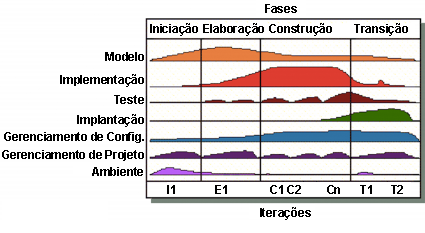
\includegraphics[width=10cm]{assets/uap} \\
\fonte{Adaptado de \citeauthoronline{edeki:13}, \citeyear{edeki:13}.}
\end{center}
\end{figure}

\subsection{Método de Desenvolvimento de Sistemas Dinâmicos (DSDM)}

O DSDM (\textit{Dynamic Systems Development Method}) ou Método de Desenvolvimento de Sistemas Dinâmicos é uma adordagem de desenvolvimento ágil utilizada para desenvolver e manter projetos de \textit{software} cujo prazo é curto. Essa metodologia surgiu em 1994 como uma demanda de líderes de empresas que estavam insatisfeitos com métodos de desenvolvimento que eram caros, rígidos e não confiáveis. Essa metodologia baseia-se na versão modificada do princípio de Pareto. Em outras palavras, a metodologia propõe que 80\% de uma aplicação pode ser entregue em 20\% do tempo que levaria para que a aplicação completa fosse feita. A metodologia utiliza o modelo iterativo de desenvolvimento (pequenas entregas) e, além disso, somente o suficiente é feito. Detalhes e requisitos obscuros são deixadas para próxima iteração. Existe um grupo chamado DSDM Consortium formado por algumas empresas que utilizam-se dessa metodologia e que ``mantêm'' o \textit{framework}. Mais informações podem ser encontradas em \textit{http://bit.ly/1JWOGIU} \cite{pressman:11} \cite{dsdm:2015}. 

O DSDM basea-se em nove princípios conforme \citeonline{macedo:12}:

\begin{itemize}
	\item Participação ativa dos usuários e \textit{stakeholders};
	\item Abordagem cooperativa e compartilhada;
	\item Equipes com poder de decisão;
	\item Entregas contínuas que fazem diferença;
	\item Desenvolvimento iterativo e incremental;
	\item \textit{Feedback};
	\item Todas as possíveis alterações durante desenvolvimento podem ser reversíveis;
	\item Fixar os requisitos essenciais e
	\item Teste em todo ciclo de vida.
\end{itemize}

Em relação aos testes, como o prazo dos projetos que utilizam-se de DSDM são rígidos, testes são feitos desde o começo (testes de regressão são bastante utilizados) \cite{macedo:12}. 

O ciclo de desenvolvimento segundo \citeonline{pressman:11} é composto por três ciclos iterativos que são precedidos por duas atividades de ciclos adicionais. São elas:

\begin{itemize}
	\item \textbf{Estudo de viabilidade}: Tem como objetivo estabelecer os requisitos básicos de negócio, restrições e a viabilidade do uso do \textit{framework} DSDM.
	\item \textbf{Estudo de negócio}: Tem como objetivo estabelecer requisitos funcionais e de informação. A arquitetura do sistema é definida também nessa etapa.
	\item \textbf{Iteração de modelos funcionais}: Tem como objetivo produzir um conjunto de protótipos funcionais que serão melhorados através do \textit{feedback} dos usuários.
	\item \textbf{Iteração de projeto e desenvolvimento}: Pode ocorrer ao mesmo tempo que a iteração de modelo funcional. Tem como objetivo revisar o que foi feito na iteração anterior e certificar-se da existência de um processo de engenharia na produção de algum valor ao negócio do cliente. 
	\item \textbf{Implementação}: É responsável por alocar o último incremento do \textit{software} no ambiente operacional. Caso o \textit{software} não esteja funcionando conforme o esperado ou venha alguma solicitação de mudança, o processo volta para a etapa de iteração de modelos funcionais.
\end{itemize}

\subsection{Desenvolvimento de Software Adaptativo (ASD)}
 
O desenvolvimento adaptativo de \textit{software} ou (\textit{adaptative software development}) é uma métodologia proposta por Sam Bayer e James Highsmith em 1997 para criação de projetos de \textit{software} de maneira mais rápida. Essa maneira mais rápida de desenvolvimento torna-se fundamental em um ambiente que exige a construção de programas complexos e em um prazo curto onde os programadores não tem muito poder de decisão \cite{pressman:11} \cite{macedo:12}. 

O ciclo da metodologia ASD possui três fases: especulação, colaboração e aprendizagem. A seguir são vistos cada um deles segundo \citeonline{pressman:11}.

Na fase de especulação há o início do projeto com o planejamento de ciclos adaptáveis. Esse planejamento envolve o levantamento de informações como: missão do cliente, restrições do projeto (e.g. data de entrega ou descrições de usuário) e requisitos básicos. Tudo isso será levantado para definição dos ciclos (incrementos) que farão parte do projeto de \textit{software}. Na etapa de colaboração é feito o levantamento de necessidades, JAD e miniespecificações. A colaboração, como parte de uma metodologia ágil, é importante e nessa metodologia não é diferente, assim gerentes de projeto e \textit{stakeholders} atuam na priorização das funcionalidades do sistema para possibilitar a organização do projeto. As funcionalidades que são mais utilizadas e importantes vão ter uma prioridade maior. O aprendizado é uma fase importante pois possibilita que todo artefato produzido seja apresentado para equipe. Revisões junto com clientes e testes são versão beta são feitas nessa etapa. Nessa fase o desenvolvedor certamente aprende cada vez mais sobre o cliente, seus desejos e os próximos passos que o projeto deve passar. Os ciclos de revisão e teste são curtos e servem apenas para aprender com erros pequenos \cite{macedo:12} \cite{pressman:11}. 

A Figura \ref{fig:asd} mostra o ciclo de desenvolvimento da metodologia. Depois da fase de aprendizado, há uma liberação de incremento de \textit{software} que é passível que sofrer ajustes para ciclos subsequentes.

\begin{figure}[htb!]
\begin{center}
\caption{Ciclo do ASD}
\label{fig:asd}
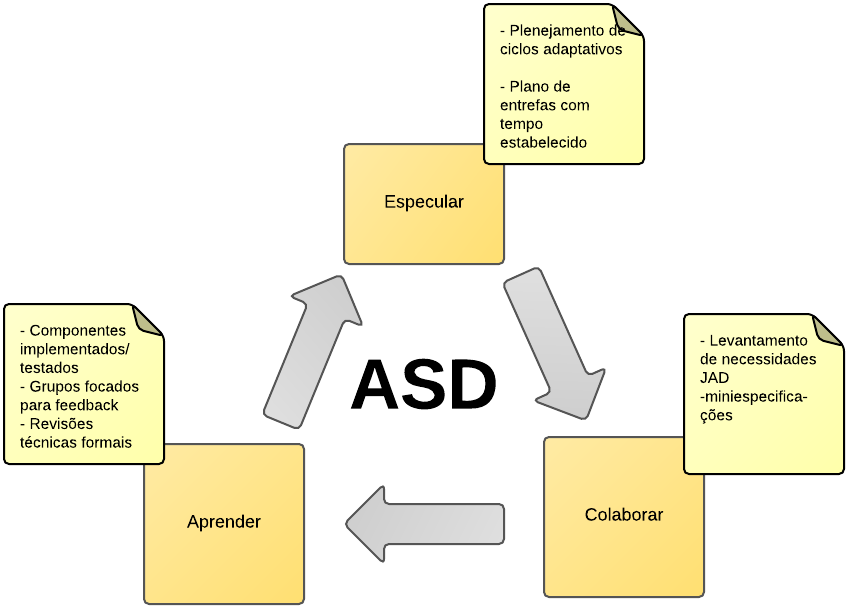
\includegraphics[width=13cm]{assets/asd} \\
\fonte{Adaptado de \citeauthoronline{pressman:11}, \citeyear{pressman:11}.}
\end{center}
\end{figure}

\subsection{Scrum}
\label{sec:scrum}

A metodologia SCRUM\footnote{O nome SCRUM é oriundo de uma atividade que acontece em uma partida de rugby.}, além de outras metodologias ágeis, foi fortemente influenciada por práticas do \textit{lean} (ou manufatura enxuta). Essa metodologia foi proposta por Jeff Sutherland e posteriormente expandida por Schwaber e Beeddle. Como uma metodologia ágil, o SCRUM é ideal para projetos cujos requisitos são incertos -- tendo assim uma grande capacidade de adaptar-se a mudanças de requisitos. Além disso, é ideal para projetos com prazo apertado. Sua principal função é orientar o desenvolvimento de \textit{software} dentro de uma processo que possui as seguintes atividades estruturais segundo \citeonline{pressman:11}:

\begin{enumerate}
	\item Requisitos;
	\item Análise;
	\item Projeto;
	\item Evolução e;
	\item Entrega.
\end{enumerate}

Em cada atividade metodológica, ocorrem tarefas que são realizadas dentro de um padrão de processo chamado de \textit{sprint}\footnote{\textit{Sprint} são corridas de velocidade em inglês.} que são iterações de trabalho com duração de duas até quatro semanas \cite{pressman:11}. 

O SCRUM é baseado segundo \citeonline{macedo:12} em seis características:

\begin{enumerate}
	\item Flexibilidade de prazos;
	\item Times pequenos;
	\item Revisões frequentes;
	\item Colaboração e
	\item Orientação a objetos;
\end{enumerate}

A Figure \ref{fig:scrumfund} mostra os fundamentos do SCRUM. Os papéis se dividem em três principais: \textit{Product Owner}, SCRUM \textit{Master} e \textit{Team} ou equipe. Além desses três papéis há a possibilidade do cliente ser incluso, pois ele exerce uma participação importante na construção do sistema. As cerimômias são reuniões que acontecem durante o ciclo de desenvolvimento do projeto e são: \textit{Daily Meeting}(ou \textit{Daily Scrum}), \textit{Sprint Review}, \textit{Sprint Planning Meeting} e \textit{Sprint Retrospective}. Os artefatos são documentos gerados através dessas reuniões ou cerimônias e são: \textit{Product Backlog}, \textit{Sprint Backlog} e \textit{Burndown Chart} \cite{macedo:12}. 

\begin{figure}[htb!]
\begin{center}
\caption{Fundamentos do SCRUM}
\label{fig:scrumfund}
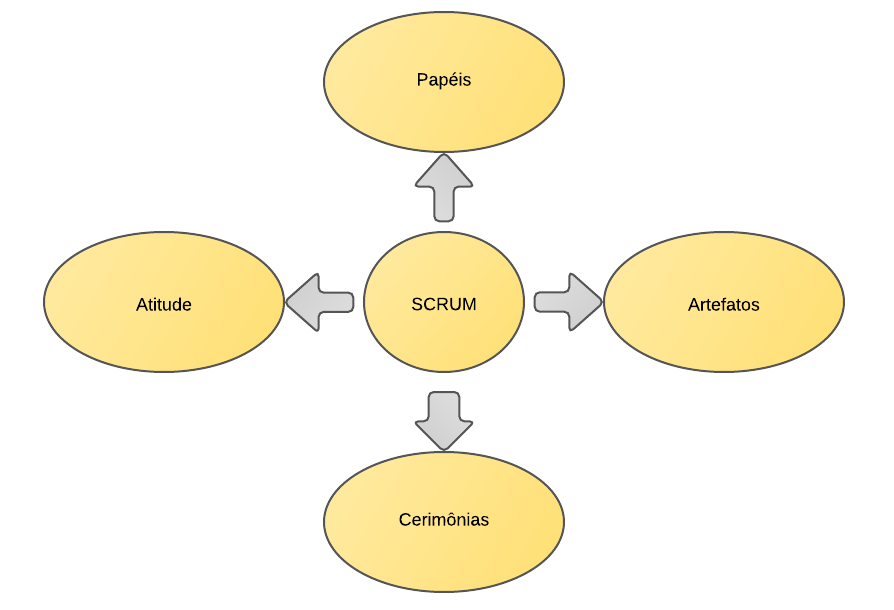
\includegraphics[width=13cm]{assets/scrum_papeis} \\
\fonte{Adaptado de \citeauthoronline{macedo:12}, \citeyear{macedo:12}.}
\end{center}
\end{figure}

O ciclo de desenvolvimento do SCRUM é mostrado na Figura \ref{fig:scrum}. Tudo começa com uma reunião entre os clientes e desenvolvedores para definição do \textit{backlog} do produto. Esse backlog de produto nada mais é do que a lista de funcionalidades que o sistema deve ter. Após acordado com o cliente sobre as entregas, riscos e prazos, é eleito o SCRUM Master entre a equipe alocada para o projeto. Com o \textit{backlog} de produto feito, é definido o que será feito na \textit{sprint}: assim é feito o \textit{backlog} de \textit{sprint} através da cerimônia de \textit{sprint planning} em que todos participam e tem duração de no máximo oito horas. Nela, o \textit{product owner} irá selecionar items do \textit{backlog} de produto e priorizar de acordo com a necessidade. Após isso, os desenvolvedores irão então quebrar as funcionalidades em atividades. Técnicas como \textit{planning poker} são utilizadas para definir o tamanho de uma atividade e medir seu esforço. O \textit{planning poker} é basicamente um jogo de cartas que os desenvolvedores utilizam para dar ``nota'' de complexidade para uma funcionalidade. Enquanto as notas das cartas divergirem entre eles, uma nova rodada é feita. A numeração de Fibonacci é geralmente empregada nesse processo. Em cada dia de trabalho é feita uma reunião (como mostra a Figura \ref{fig:scrum}) chamada de \textit{daily scrum} entre o SCRUM Master e o Time de no máximo 15 minutos cujo objetivo principal é saber o que cada um está fazendo, o que será feito hoje, se há algum impedimento e quais. Ao final de 2 a 4 semanas tem-se um incremento de \textit{software}. Ao final da \textit{sprint} é realizada a cerimônia de \textit{sprint review} cujo objetivo é mostrar os resultados da \textit{sprint} para o \textit{Product Owner} e outras pessoas convidadas. A cerimônia de retrospectiva de \textit{sprint} ou \textit{retrospective sprint} é também realizada com a participação do time e SCRUM master. O \textit{product owner} pode estar presente, embora sua participação não seja obrigatória. Essa cerimônia tem como objetivo ver o que deu certo e o que deu errado para melhorar as próximas \textit{sprints} \cite{macedo:12} \cite{cohn:11}. 

\begin{figure}[htb!]
\begin{center}
\caption{Dinâmica do SCRUM}
\label{fig:scrum}
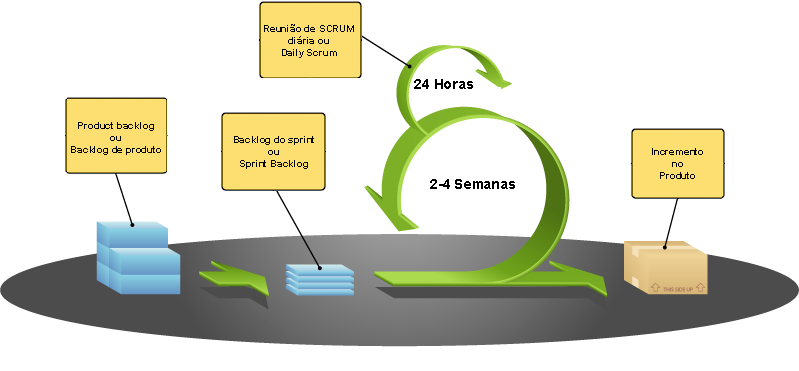
\includegraphics[width=15cm]{assets/scrum} \\
\fonte{Adaptado de \citeauthoronline{macedo:12}, \citeyear{macedo:12}.}
\end{center}
\end{figure}

Alguns artefatos produzidos, como mencionado anteriormente, com o SCRUM são \textit{backlog} de produto, \textit{backlog} de \textit{sprint}, \textit{task board} (utilizado mapear o estado das atividades na sprint) e o gráfico Burndown que é feito pelo SCRUM Master para verificar o esforço de cada interação e fazer o acompanhamente de forma gráfica \cite{macedo:12}. 

\subsection{Desenvolvimento de Software Enxuto (LSD)}

O desenvolvimento de \textit{software} enxuto ou LSD (\textit{lean software development}) é uma metodologia de desenvolvimento que visa aplicar os princípios da fabricação enxuta para a engenharia de \textit{software}. Os princípios que norteiam o LSD e que vieram do pensamento \textit{lean} são:

\begin{itemize}
	\item Eliminiar desperdício;
	\item Incorporar qualidade;
	\item Criar conhecimento;
	\item Adiar compromisso;
	\item Engregar rápido;
	\item Respeitar as pessoas e
	\item Otimizar o todo.
\end{itemize}

O LSD adapta cada princípio do pensamento \textit{lean} ao processo de \textit{software}. Para eliminar desperdício pode-ser executar as seguintes acões segundo \citeonline{pressman:11}:

\begin{enumerate}
	\item Não adicionar recursos ou funções que possivelmente não serão percebidas ou utilizadas pelos usuários;
	\item Avaliar o impacto do custo e do cronograma de qualquer requisito solicitado;
	\item Eliminar qualquer etapa de processo que não seja realmente necessária;
	\item Estabelecer mecanismos para elicitação de requisitos;
	\item Escrever e executar testes de qualidade;
	\item Reduzir tempo para solicitar e receber uma decisão que afete o \textit{software} e
	\item Racionalizar o fluxo de informação entre as pessoas envolvidas no processo
\end{enumerate}

No próximo capítulo é abordada essa metodologia com mais detalhes. 

\section{CONCLUSÃO DO CAPÍTULO}

As pessoas envolvidas com o desenvolvimento de \textit{software} sempre procuraram melhorar a entrega em termos de prazo, custo e qualidade e assim novos modelos foram sendo criados e adaptados para melhorar o processo de desenvolvimento. Toda essa evolução e criação de novos processos foram importantes para o entendimento da natureza do \textit{software}, que ao contrário das outras engenharias é fruto de um trabalho social que envolve a participação massiva do cliente: principalmente nas metodologias ágeis. Pode-se dizer que não existe uma metologia de processo melhor ou pior e que tudo vai depender do tipo de projeto e complexidade. O modelo RUP, embora completo, não seria ideal para o desenvolvimento de um sistema simples, devido ao seu custo maior de implantação por exemplo. Dependendo da empresa, um ou outro processo se torna mais ideal para uma equipe de desenvolvimento. No caso do SCRUM, por exemplo, é essencial que todas as pessoas da equipe estejam sempre motivadas e sejam ágeis o suficiente para se adaptar a mudanças no projeto e isso não se adquire de uma hora para outra. Além disso, a comunicação entre todas as pessoas é essencial (principalemte com o cliente). O próximo capítulo aborda melhor o desenvolvimento enxuto de \textit{software} ou LSD (\textit{lean software development}).